\documentclass[10pt,a4paper]{article}

\usepackage[a4paper, top=0.9cm, bottom=0.9cm, left=1cm, right=1cm]{geometry}
\usepackage{graphicx}
\usepackage{float}
\usepackage{amsmath}
\usepackage{amssymb}
\usepackage[table]{xcolor}
\usepackage{mdframed}
\usepackage{parskip}
\usepackage{enumitem}
\usepackage{titlesec}
\usepackage{booktabs}
\usepackage{array}
\usepackage{tikz}
\usetikzlibrary{arrows.meta, positioning}
\usepackage[T1]{fontenc}

% ── Colours ────────────────────────────────────────────────────────────────
\definecolor{keyblue}{RGB}{30, 80, 160}
\definecolor{keybluebg}{RGB}{220, 235, 255}
\definecolor{noteorange}{RGB}{200, 100, 0}
\definecolor{noteorangebg}{RGB}{255, 240, 215}
\definecolor{warnred}{RGB}{180, 30, 30}
\definecolor{warnredbg}{RGB}{255, 220, 220}
\definecolor{defgreen}{RGB}{20, 110, 50}
\definecolor{defgreenbg}{RGB}{215, 245, 225}
\definecolor{headernavy}{RGB}{25, 35, 90}

\newmdenv[linecolor=keyblue,backgroundcolor=keybluebg,linewidth=1.5pt,
  leftline=true,rightline=false,topline=false,bottomline=false,
  innerleftmargin=7pt,innerrightmargin=6pt,
  innertopmargin=3pt,innerbottommargin=3pt,
  skipabove=3pt,skipbelow=3pt]{keybox}

\newmdenv[linecolor=noteorange,backgroundcolor=noteorangebg,linewidth=1.5pt,
  leftline=true,rightline=false,topline=false,bottomline=false,
  innerleftmargin=7pt,innerrightmargin=6pt,
  innertopmargin=3pt,innerbottommargin=3pt,
  skipabove=3pt,skipbelow=3pt]{notebox}

\newmdenv[linecolor=defgreen,backgroundcolor=defgreenbg,linewidth=1.5pt,
  leftline=true,rightline=false,topline=false,bottomline=false,
  innerleftmargin=7pt,innerrightmargin=6pt,
  innertopmargin=3pt,innerbottommargin=3pt,
  skipabove=3pt,skipbelow=3pt]{defbox}

\newmdenv[linecolor=warnred,backgroundcolor=warnredbg,linewidth=1.5pt,
  leftline=true,rightline=false,topline=false,bottomline=false,
  innerleftmargin=7pt,innerrightmargin=6pt,
  innertopmargin=3pt,innerbottommargin=3pt,
  skipabove=3pt,skipbelow=3pt]{warnbox}

\titleformat{\section}[block]{\normalsize\bfseries\color{headernavy}}{}{0pt}{}
  [\vspace{1pt}\rule{\linewidth}{0.6pt}\vspace{2pt}]
\titleformat{\subsection}[block]{\small\bfseries\color{keyblue}}{}{0pt}{}
\titlespacing*{\section}{0pt}{5pt}{2pt}
\titlespacing*{\subsection}{0pt}{3pt}{1pt}

\setlist{nosep, topsep=1pt, itemsep=1pt, leftmargin=1.3em}
\parskip=2pt
\parindent=0pt

% ===========================================================================
\begin{document}
% ===========================================================================

\begin{center}
  {\large\bfseries\color{headernavy} Q4 \textemdash{} Network Calculus \& RTC Toolbox}\\[1pt]
  {\small MM4/5 $\cdot$ Hans-Peter Schwefel}
\end{center}
\vspace{1pt}\hrule height 1pt\vspace{5pt}

Network Calculus is used to give \textbf{deterministic worst-case bounds} by modelling traffic as:
\begin{itemize}
\item \textbf{arrival curves} and link capacity as \textbf{service curves}
\end{itemize}  
No probability needed. It answers:
\begin{itemize}
  \item \textbf{Delay} --- how long can a packet wait in the worst case?
  \item \textbf{Backlog} --- how full can the buffer get in the worst case?
\end{itemize}

% ===========================================================================
\section*{1\quad Core Concepts}
% ===========================================================================

\subsection*{Arrival Curve $\alpha(t)$}
Upper bound on the number of bits arriving in any window of length $t$, modelled as an affine linear \textbf{token bucket}:
\[
  \alpha(t) = r \cdot t + b
\]
\begin{itemize}
  \item $r$ --- long-term sustained rate [kbps]
  \item $b$ --- burst size [bits]: max bits that can arrive instantly
  \item meaning: at most $b$ bits spike at $t{=}0$, then arrivals grow at rate $r$
\end{itemize}

\subsection*{Service Curve $\beta(t)$}
Lower bound on bits served in any window of length $t$, modelled as a pure-rate link:
\[
  \beta(t) = C \cdot t
\]
\begin{itemize}
  \item $C$ --- link capacity [kbps]
\end{itemize}
  \begin{warnbox}
    \begin{itemize}
      \item \textbf{Note That we need arrival rate $r$ to be lower then link capacity $C$}
  \item $\rho = r/C$ --- utilisation; system \textbf{stable} if $\rho < 1$
  \item if $r = C$: curves run parallel, delay is finite ($= b/C$) but queue never fully drains
  \end{itemize}  
\end{warnbox}
% ===========================================================================
\section*{2\quad Exercise 2 --- Sensor Network RTC Analysis}
% ===========================================================================

\textbf{System:} 8 sensors each producing 100\,bits/sample every 1\,ms:
\begin{itemize}
  \item packetised into packets of $N$ data samples $+$ 100\,bits overhead $\Rightarrow$ $L = 100N + 100$ bits
  \item all 8 sensors share a single \textbf{1\,Mbps} link
\end{itemize}

\subsection*{From Exercise 1 --- why $N=4$}
From Exercise 1 the goal was to find $N$ that maximises link utilisation without exceeding capacity. The \textbf{aggregate rate} across 8 sensors is:
\[ r_{\text{agg}} = \frac{8(100N+100)}{N}\;\text{kbps} \]
\begin{itemize}
  \item $N$ --- number of data samples per packet
  \item $100N + 100$ --- packet length $L$ in bits ($N$ samples + 100\,bits overhead)
  \item $N$ in denominator --- inter-packet period per sensor grows with $N$ [ms]
\end{itemize}
\begin{notebox}
\begin{itemize}
  \item At $N=3$: $r_{\text{agg}} \approx 1067\,\text{kbps} > 1000$ $\Rightarrow$ unstable
  \item At $N=4$: $r_{\text{agg}} = 1000\,\text{kbps} = C$, $\rho = 1$ $\Rightarrow$ boundary (finite delay)
\end{itemize}
Both as also observed in the $N$ sweep table below. \\
\end{notebox}
\subsection*{Exercise 2 --- Arrival \& Service Curves}
We model the aggregate traffic as a \textbf{token bucket} and the link as a \textbf{pure-rate service curve}:
\begin{itemize}
  \item \textbf{Burst} $b_{\text{agg}} = 8 \cdot L$ --- worst case: all 8 sensors have one packet ready simultaneously at $t=0$
  \item \textbf{Rate} $r_{\text{agg}} = 8 \cdot L/P$ --- aggregate sustained sending rate [kbps]
\end{itemize}
We use three RTC toolbox functions:
\begin{itemize}
  \item \texttt{rtccurve([[0 b r]])} \quad --- encode an affine token-bucket curve with burst $b$ and rate $r$
  \item \texttt{rtch($\alpha$, $\beta$)} \quad\quad\quad\quad\quad\;\; --- max \emph{horizontal} distance $\Rightarrow$ \textbf{worst-case delay}
  \item \texttt{rtcv($\alpha$, $\beta$)} \quad\quad\quad\quad\quad \;\; --- max \emph{vertical} distance $\Rightarrow$ \textbf{worst-case backlog}
\end{itemize}

\begin{keybox}
\textbf{How $r$ vs.\ $C$ determines the result:}
\begin{itemize}
  \item $r > C$: arrival rate exceeds link $\Rightarrow$ \textbf{unstable}, delay $= \infty$, backlog $= \infty$
  \item $r = C$: curves run parallel, constant gap forever $\Rightarrow$ delay $= b/C$, backlog $= b$ (never drains)
  \item $r < C$: worst case at $t{=}0$, then gap shrinks $\Rightarrow$ delay $= b/(C-r)$, backlog $= b$ (eventually drains)
\end{itemize}
\end{keybox}

\vspace{4pt}
\clearpage
\begin{minipage}[t]{0.52\textwidth}
\subsection{N sweep results (link $s = 1000$\,kbps)}
\vspace{2pt}
\begin{tabular}{@{}c|r|r|r|r|r@{}}
\toprule
$N$ & $L$ [bits] & $r_{\text{agg}}$ [kbps] & $\rho$ & Delay [ms] & Backlog [bits] \\\midrule
1 & 200 & 1600 & 1.600 & $\infty$ & $\infty$ \\
2 & 300 & 1200 & 1.200 & $\infty$ & $\infty$ \\
3 & 400 & 1067 & 1.067 & $\infty$ & $\infty$ \\
\rowcolor{defgreenbg}
4 & 500 & 1000 & 1.000 & \textbf{4.0} & 4000 \\
5 & 600 &  960 & 0.960 & 15.0 & 4800 \\
6 & 700 &  933 & 0.933 & 8.75 & 5600 \\
7 & 800 &  914 & 0.914 & 9.33 & 6400 \\
8 & 900 &  900 & 0.900 & 7.20 & 7200 \\\bottomrule
\end{tabular}
\end{minipage}\hfill
\begin{minipage}[t]{0.36\textwidth}
\vspace{3pt}
\begin{keybox}
\textbf{Optimal $N=4$:} minimum $N$
\begin{itemize}
\item finite delay
\item $r_{\text{agg}} = C$ is boundary --- curves parallel 
\item delay $= b/C = 4000/1000 = 4\,\text{ms}$, finite
\end{itemize} 
$N=3$ is unstable ($r > C$, delay $\to \infty$).\\
\textbf{Practical choice: $N=5$} 
\begin{itemize}
\item gives 40\,kbps spare capacity
\item delay $= b/(C-r) = 4800/40 = 120\,\text{ms}$
\item -- acceptable headroom.
\end{itemize}
\end{keybox}
\end{minipage}

% ===========================================================================
\section*{3\quad Exercise 3 --- CAN Bus with Priority Scheduling}
% ===========================================================================
We are told to model a CAN bus with 3 nodes using \textbf{priority scheduling} --- lower CAN-ID wins arbitration (from Q2). First we determine the minimum bitrate, then build the RTC model. \\[4pt]
The Tree nodes are:
\begin{center}
\begin{tabular}{@{}l|c|c|c@{}}
Node & Period & CAN-ID & Priority \\\midrule
0 & 2\,ms & 0x000 & Highest \\
1 & 5\,ms & 0x001 & Middle \\
2 & 3\,ms & 0x002 & Lowest \\
\end{tabular} \\
\end{center}

\begin{keybox}
\textbf{Min bitrate} --- each node must fit at least one packet per period:
\[ C_{\min} = L\!\left(\tfrac{1}{T_0}+\tfrac{1}{T_1}+\tfrac{1}{T_2}\right) = 100\!\left(\tfrac{1}{2}+\tfrac{1}{5}+\tfrac{1}{3}\right) \approx 103.3\;\text{kbps} \]
Choose any $C > C_{\min}$; exercise uses $C = 200$\,kbps.
\end{keybox}

\subsection*{Priority Server Theory}
\begin{minipage}[t]{0.52\textwidth}
High priority gets the \textbf{full} service; low priority gets only the \textbf{residual}:
\begin{itemize}
  \item $\sigma_H = \sigma$ \quad --- high-priority gets the full service curve
  \item $\sigma_L = [\sigma - \alpha_H]^+$ \quad --- low-priority gets residual; $[\cdot]^+$ clamps to zero (cannot go negative)
  \item \textbf{Non-preemptive} (CAN): once a packet starts it \emph{cannot} be interrupted --- low-priority must wait for any in-progress packet to finish
\end{itemize}
\end{minipage}\hfill
\begin{minipage}[t]{0.44\textwidth}
\vspace{0pt}
\centering
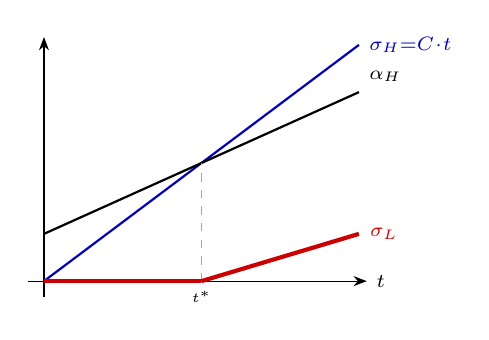
\begin{tikzpicture}[>=Stealth, font=\scriptsize, scale=1.0]
  % Axes
  \draw[->] (-0.2,0) -- (4.1,0) node[right] {$t$};
  \draw[->] (0,-0.2) -- (0,3.1);
  % sigma_H = C*t  (slope 0.75)
  \draw[thick, blue!70!black] (0,0) -- (4.0,3.0)
    node[right, font=\scriptsize] {$\sigma_H{=}C\!\cdot\!t$};
  % alpha_H: burst b=0.6 at t=0, then slope r=0.45
  %   token-bucket vertical jump then linear
  \draw[thick, black] (0,0) -- (0,0.6);
  \draw[thick, black] (0,0.6) -- (4.0, 2.4)
    node[above right, font=\scriptsize] {$\alpha_H$};
  % Intersection: 0.75t = 0.45t+0.6 => t*=2.0, y=1.5
  \draw[dashed, gray!70] (2.0,0) -- (2.0,1.5);
  \node[below, font=\tiny] at (2.0,0) {$t^*$};
  % sigma_L = [sigma_H - alpha_H]+  (red)
  %   0 for t<2, then (0.75-0.45)t - 0.6 = 0.3t-0.6
  \draw[red!80!black, line width=1.5pt] (0,0) -- (2.0,0);
  \draw[red!80!black, line width=1.5pt] (2.0,0) -- (4.0,0.6)
    node[right, font=\scriptsize, red!80!black] {$\sigma_L$};
\end{tikzpicture}
\vspace{2pt}
\small$\sigma_L$ is what is \emph{left} of the bus capacity after $\alpha_H$ has consumed its share --- the low-priority node can only use the shaded residual.
\end{minipage}

\subsection*{CAN GPC Chain}
Because each node degrades the service for the next, both the \textbf{output arrival curve} ($\alpha^*$, shaped by the GPC) and the \textbf{residual service curve} ($\sigma^*$, reduced after each node) change at every stage in the chain:\\ 
\begin{minipage}[t]{0.36\textwidth}
\vspace{0pt}
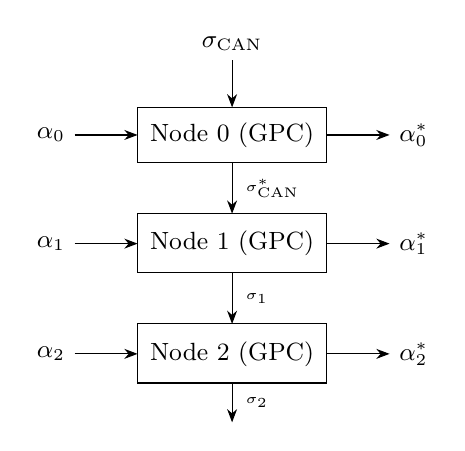
\begin{tikzpicture}[>=Stealth, font=\small]
  % Node 0
  \draw (0.8,4.8) rectangle (3.2,5.5);
  \node at (2.0,5.15) {\small Node 0 (GPC)};
  \draw[->] (2.0,6.1) -- (2.0,5.5); \node[above] at (2.0,6.1) {$\sigma_{\text{CAN}}$};
  \draw[->] (0.0,5.15) -- (0.8,5.15); \node[left] at (0.0,5.15) {$\alpha_0$};
  \draw[->] (3.2,5.15) -- (4.0,5.15); \node[right] at (4.0,5.15) {$\alpha_0^*$};
  \draw[->] (2.0,4.8) -- (2.0,4.15); \node[right,font=\tiny] at (2.05,4.47) {$\sigma_{\text{CAN}}^*$};
  % Node 1
  \draw (0.8,3.4) rectangle (3.2,4.15);
  \node at (2.0,3.77) {\small Node 1 (GPC)};
  \draw[->] (0.0,3.77) -- (0.8,3.77); \node[left] at (0.0,3.77) {$\alpha_1$};
  \draw[->] (3.2,3.77) -- (4.0,3.77); \node[right] at (4.0,3.77) {$\alpha_1^*$};
  \draw[->] (2.0,3.4) -- (2.0,2.75); \node[right,font=\tiny] at (2.05,3.07) {$\sigma_1$};
  % Node 2
  \draw (0.8,2.0) rectangle (3.2,2.75);
  \node at (2.0,2.37) {\small Node 2 (GPC)};
  \draw[->] (0.0,2.37) -- (0.8,2.37); \node[left] at (0.0,2.37) {$\alpha_2$};
  \draw[->] (3.2,2.37) -- (4.0,2.37); \node[right] at (4.0,2.37) {$\alpha_2^*$};
  \draw[->] (2.0,2.0) -- (2.0,1.5); \node[right,font=\tiny] at (2.05,1.75) {$\sigma_2$};
\end{tikzpicture}
\end{minipage}\hfill
\begin{minipage}[t]{0.60\textwidth}
\begin{notebox}
\small\textbf{Arrival \& service curve types:}\\
Periodic nodes $\Rightarrow$ \textbf{token bucket} (affine) arrival curves:\\[1pt]
\texttt{rtccurve([[0, L, L/T\_i]])} \quad $r = L/T$, $b = L$\\[3pt]
CAN bus service: \texttt{rtcbdu(0,C)} / \texttt{rtcbdl(0,C)}\\[2pt]
$\sigma_{\text{CAN}} = C\cdot t$ (strict), $\alpha_{\text{HoL}}=k$ (one blocking packet)\\[4pt]
\textbf{Token bucket = staircase (MM4 Prop 1.2.2):} for fixed-size packets with period $T$ and no jitter ($\tau{=}0$): $r=L/T$, $b=L$ gives \emph{identical} bounds --- the two forms are mathematically equivalent.
\end{notebox}
\vspace{3pt}
\begin{keybox}
\small\textbf{GPC chain --- each node gets the residual of the previous:}
\begin{enumerate}[leftmargin=1.5em, itemsep=1pt]
  \item \texttt{rtcgpc($\alpha_0$, $\beta$, L)} $\;\to\;$ $\alpha_0^*$,\, $\sigma^*_{\text{CAN}}$,\, del0
  \item \texttt{rtcgpc($\alpha_1$, $\sigma^*_{\text{CAN}}$, L)} $\;\to\;$ $\alpha_1^*$,\, $\sigma_1$,\, del1
  \item \texttt{rtcgpc($\alpha_2$, $\sigma_1$, L)} $\;\to\;$ $\alpha_2^*$,\, $\sigma_2$,\, del2
\end{enumerate}
Node 2 waits for both 0 \& 1 $\Rightarrow$ largest delay and buffer.
\end{keybox}
\end{minipage}
\end{document}
